
\definecolor{ceeffaa}{RGB}{238,255,170}
\definecolor{c0000ff}{RGB}{0,0,255}
\definecolor{c008080}{RGB}{0,128,128}
\definecolor{c008000}{RGB}{0,128,0}
\definecolor{cd40000}{RGB}{212,0,0}

\resizebox {0.5\textwidth} {!} {
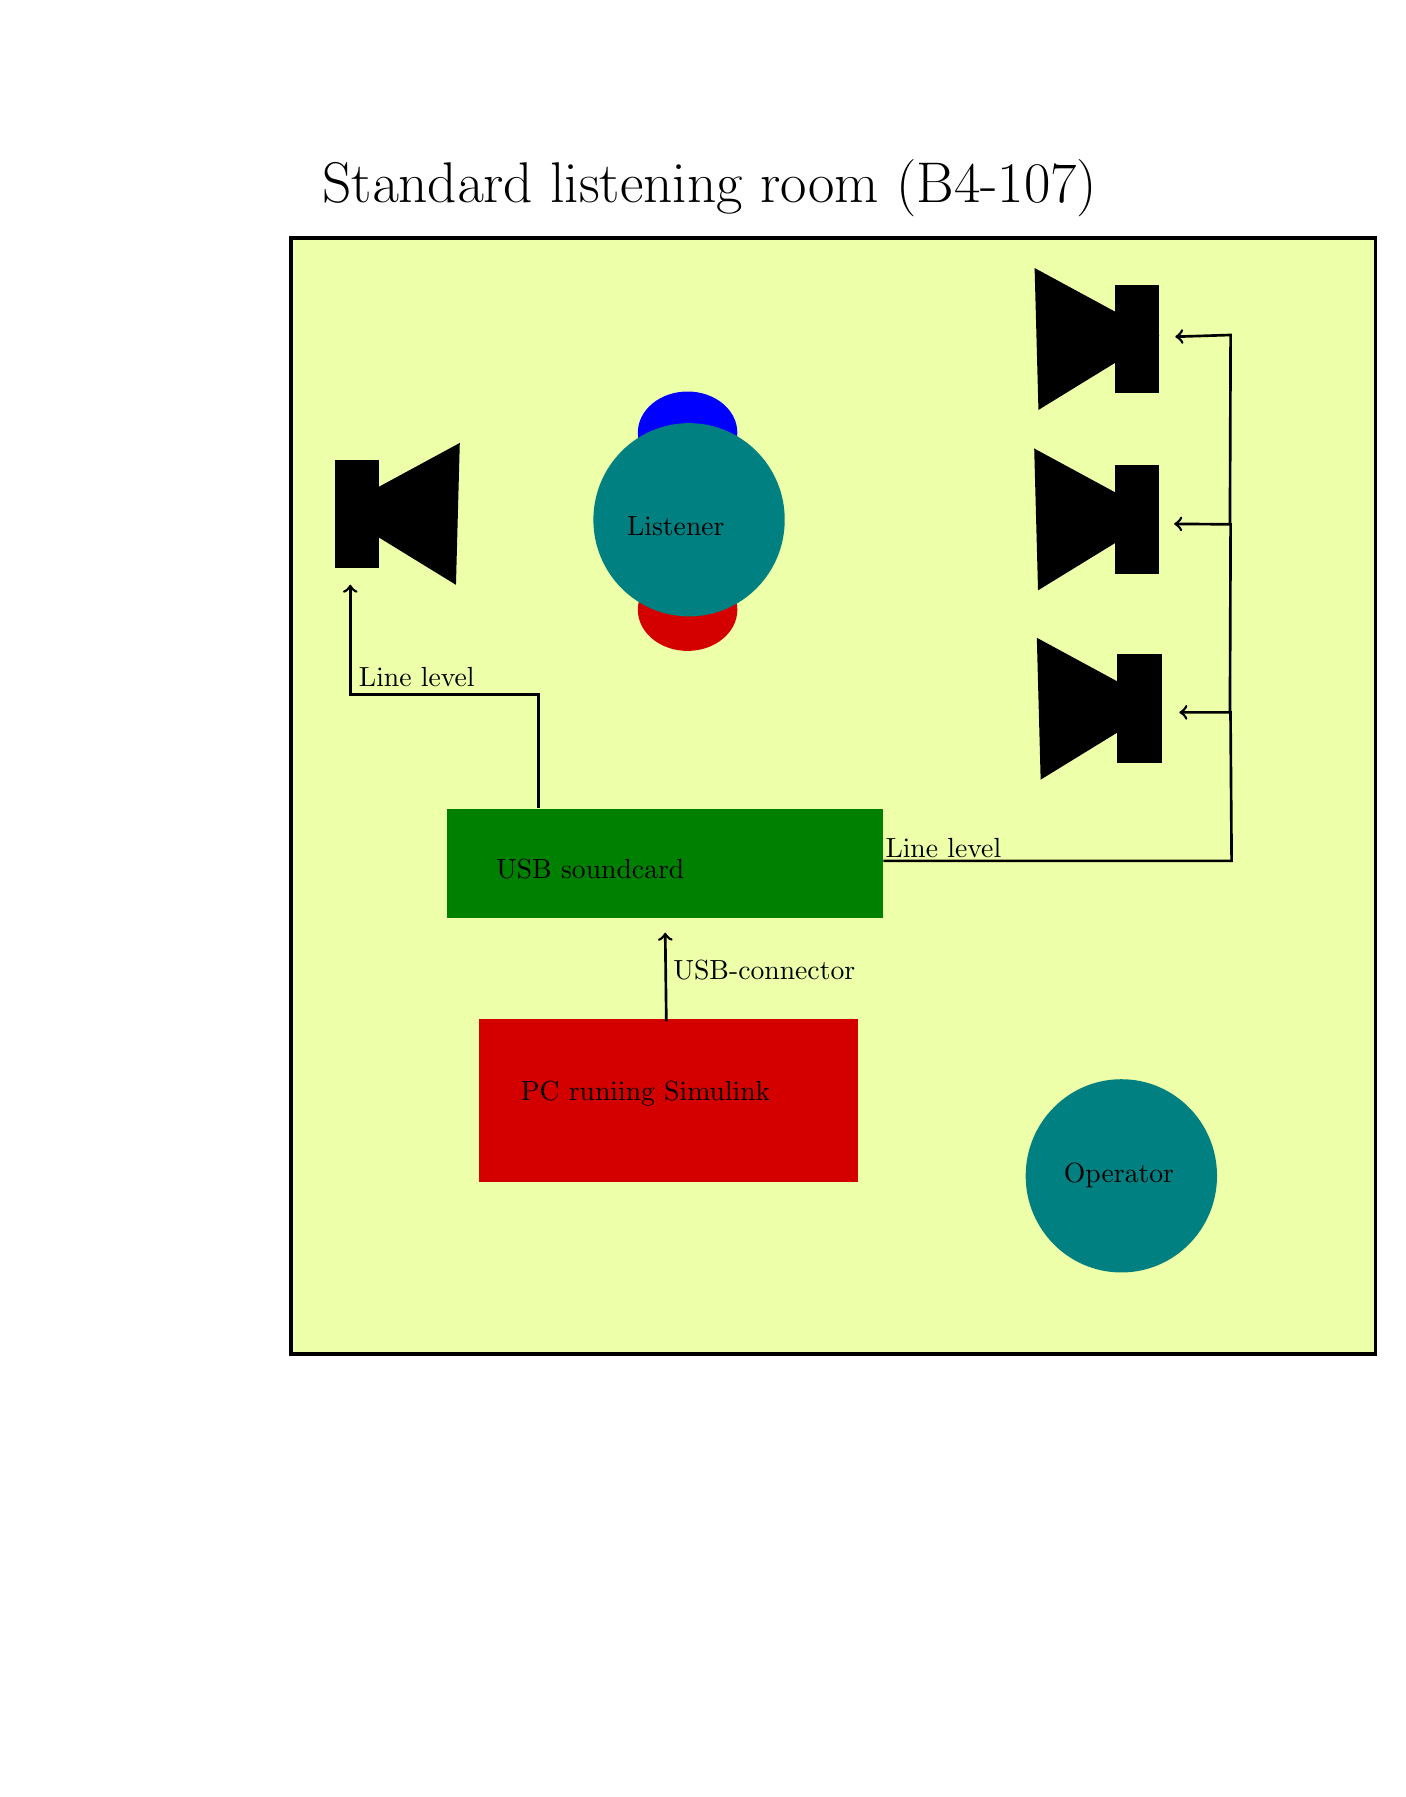
\begin{tikzpicture}[y=0.80pt, x=0.80pt, yscale=-1.000000, xscale=1.000000, inner sep=0pt, outer sep=0pt]
\begin{scope}[shift={(-200,-200)}]% layer1
  % rect3342
  \path[draw=black,fill=ceeffaa,line join=miter,line cap=butt,even odd rule,line
    width=1.418pt,rounded corners=0.0000cm] (118.8611,93.6237) rectangle
    (608.7849,597.9682);

  % path3348-0
  \path[cm={{0.0,-1.0,1.0,0.0,(0.0,0.0)}},fill=c0000ff] (-181.6738,298.0701)
    ellipse (0.5225cm and 0.6318cm);

  % path3348-0
  \path[cm={{0.0,-1.0,1.0,0.0,(0.0,0.0)}},fill=cd40000] (-261.6738,298.0701)
  ellipse (0.5225cm and 0.6318cm);

  % text3399
  \path[xscale=0.924,yscale=1.083,fill=black,line join=miter,line cap=butt,line
    width=0.800pt] (144.1745,77.7213) node[above right] (text3399) {\huge{Standard
    listening room (B4-107)}};

  % path3350-7
  \path[fill=c008080] (298.7422,221.0265) ellipse (1.2151cm and 1.2272cm);

  % text3494
  \path[fill=black,line join=miter,line cap=butt,line width=0.800pt]
    (270.7353,228.2140) node[above right] (text3494) {Listener};

  % text4346
  \path[fill=black,line join=miter,line cap=butt,line width=0.800pt]
    (515.8203,272.6747) node[above right] (text4346) {};

  % text4387
  \path[fill=black,line join=miter,line cap=butt,line width=0.800pt]
    (285.9375,785.1747) node[above right] (text4387) {};

  % path3350-7-3
  \path[fill=c008080] (494.0000,517.3622) ellipse (1.2151cm and 1.2272cm);

  % text3458
  \path[fill=black,line join=miter,line cap=butt,line width=0.800pt]
    (487.0000,433.3622) node[above right] (text3458) {};

  % text3494-3
  \path[fill=black,line join=miter,line cap=butt,line width=0.800pt]
    (468.0499,522.7723) node[above right] (text3494-3) {Operator};

  % rect3480
  \path[fill=black,rounded corners=0.0000cm] (491.0000,196.3622) rectangle
    (511.0000,245.3622);

  % path3498
  \path[fill=black] (511.0000,219.3622) -- (483.6830,236.1337) --
    (456.3660,252.9051) -- (455.5000,220.8622) -- (454.6340,188.8193) --
    (482.8170,204.0907) -- cycle;

  % rect3480-8
  \path[fill=black,rounded corners=0.0000cm] (492.1830,281.8622) rectangle
    (512.1830,330.8622);

  % path3498-4
  \path[fill=black] (512.1830,304.8622) -- (484.8660,321.6337) --
    (457.5490,338.4052) -- (456.6830,306.3622) -- (455.8170,274.3193) --
    (484.0000,289.5907) -- cycle;

  % rect3480-2
  \path[fill=black,rounded corners=0.0000cm] (491.1830,114.8622) rectangle
    (511.1830,163.8622);

  % path3498-0
  \path[fill=black] (511.1830,137.8622) -- (483.8660,154.6337) --
    (456.5490,171.4051) -- (455.6830,139.3622) -- (454.8170,107.3193) --
    (483.0000,122.5907) -- cycle;

  % rect3480-2-3
  \path[xscale=-1.000,yscale=1.000,fill=black,rounded corners=0.0000cm]
    (-158.8170,193.8622) rectangle (-138.8170,242.8622);

  % path3498-0-7
  \path[xscale=-1.000,yscale=1.000,fill=black] (-138.8169,216.8622) --
    (-166.1339,233.6337) -- (-193.4509,250.4051) -- (-194.3170,218.3622) --
    (-195.1830,186.3193) -- (-167.0000,201.5907) -- cycle;

  % rect3575
  \path[fill=c008000,rounded corners=0.0000cm] (189.5000,351.7958) rectangle
    (386.5000,400.7958);

  % text3577
  \path[fill=black,line join=miter,line cap=butt,line width=0.800pt]
    (239.0000,451.3622) node[above right] (text3577) {};

  % text3494-3-1
  \path[fill=black,line join=miter,line cap=butt,line width=0.800pt]
    (211.5889,382.9911) node[above right] (text3494-3-1) {USB soundcard};

  % rect3599
  \path[fill=cd40000,rounded corners=0.0000cm] (203.6543,446.3622) rectangle
    (375.0000,520.3622);

  % text3494-3-1-8
  \path[fill=black,line join=miter,line cap=butt,line width=0.800pt]
    (222.7266,485.8085) node[above right] (text3494-3-1-8) {PC runiing Simulink};

  % path5039
  \path[draw=black,line join=miter,line cap=butt,miter limit=4.00,even odd
    rule,line width=0.960pt,->] (230.6060,351.1937) -- (230.6060,299.8080) --
    (145.7094,299.8080) -- (145.7094,250.3569);

  % path5039-1
  \path[draw=black,line join=miter,line cap=butt,miter limit=4.00,even odd
    rule,line width=0.960pt,->] (386.5000,375.1037) -- (543.8028,375.1037) --
    (543.3028,308.0104) -- (520.1837,308.0104);

  % path4417
  \path[draw=black,line join=miter,line cap=butt,miter limit=4.00,even odd
    rule,line width=0.960pt,->] (543.0462,308.5833) -- (543.3507,223.0833) --
    (517.8507,222.8772);

  % path4417-2
  \path[draw=black,line join=miter,line cap=butt,miter limit=4.00,even odd
    rule,line width=0.960pt,->] (543.0462,223.0554) -- (543.3507,137.5554) --
    (518.3507,138.3493);

%  % path4417-7
%  \path[draw=black,line join=miter,line cap=butt,miter limit=4.00,even odd
%    rule,line width=0.960pt] (40.9335,91.5258) -- (41.2380,6.0258) --
%    (6.7380,5.8196);

  % path14264
  \path[draw=black,fill=black,line join=miter,line cap=butt,miter limit=4.00,even
    odd rule,line width=0.960pt,<-] (287.9691,407.5337) -- (288.4691,447.5337);

  % text3494-7
  \path[fill=black,line join=miter,line cap=butt,line width=0.800pt]
    (387.4732,373.4401) node[above right] (text3494-7) {Line level};

  % text3494-7-7
  \path[fill=black,line join=miter,line cap=butt,line width=0.800pt]
    (149.6416,296.3329) node[above right] (text3494-7-7) {Line level};

  % text3494-7-77
  \path[fill=black,line join=miter,line cap=butt,line width=0.800pt]
    (291.6416,428.8329) node[above right] (text3494-7-77) {USB-connector};

  % flowRoot3471
  \path[fill=black,line join=miter,line cap=butt,line width=0.800pt]
    (0.0000,0.0000) node[above right] (flowRoot3471) {};

\end{scope}

\end{tikzpicture}}

